% ==== 原文 p.24 ====
\section{希尔伯特空间结构}\label{sec:4}

% [Tutor Note: 本节重点] 物理图像/数学工具/主要结论
\begin{keytakeaways}
\begin{itemize}[leftmargin=1.4em,itemsep=2pt,topsep=2pt]
  \item \textbf{物理图像：}把 3 维流形 $M$ 沿曲面 $\Sigma$ 切开，理论就化成 $\Sigma\times\R$ 上的正则量子化：$\R$ 是时间，$\Sigma$ 是“空间”。$\Sigma$ 的拓扑只允许有限多个非平凡威尔逊圈，相空间因而缩成紧致、有限体积的平坦联络模空间，量子化得到的希尔伯特空间是有限维的。
  \item \textbf{数学工具：}平坦联络模空间 $\mathcal{M}$（Atiyah--Bott 的维数与奇点分析）、几何量子化与全纯量子化、前量子线丛与陈联络、行列式线丛（Quillen 的 $\bar\partial$ 行列式）、小平嵌入定理、模函子（Segal）。
  \item \textbf{主要结论：}$\mathcal{H}_\Sigma$ 是紧凯勒模空间 $\mathcal{M}_J$ 上某条正线丛的全纯截面空间，故有限维；$k=1$、$G=\mathrm{SU}(N)$ 时这条线丛正是 $\bar\partial$ 的行列式线丛，一般能级与一般群则取它的张量幂；$\mathcal{H}_\Sigma$ 不依赖复结构 $J$，$\Sigma\mapsto\mathcal{H}_\Sigma$ 构成一个模函子。
\end{itemize}
\end{keytakeaways}

% [Tutor Note: 易错点] p.24--p.28 上同一字母有多种写法：3 维流形 $M$、平坦联络模空间 $\mathcal{M}$、固定复结构的 $\mathcal{M}_J$、黎曼面模空间 $\mathcal{M}_\Sigma$；相空间另记 $\mathcal{P}$，希尔伯特空间记 $\mathcal{H}_\Sigma$。
\begin{yizhu}[易错点]
从本节起，同一字母有多种写法，务必按上下文分清：3 维流形用普通体 $M$（原文 “the 3-manifold $M$”）；平坦联络模空间用花体 $\mathcal{M}$（原文 “the resulting phase space $\mathcal{M}$”）；选定复结构后写 $\mathcal{M}_J$；$\Sigma$ 上复结构本身的模空间写 $\mathcal{M}_\Sigma$。相空间记 $\mathcal{P}$，希尔伯特空间记 $\mathcal{H}_\Sigma^{(J)}$，二者都不是 $M$。原文 $M$ 与 $\mathcal{M}$ 在版面上只差一个花体，读 p.24--p.28 时须逐处确认。
\end{yizhu}

\paragraph{开战}
% 原文标题：Into the fray.
这一节，我们放下路径积分，去承担一个雄心勃勃的目标：精确求解陈--西蒙斯理论。所谓“求解”，就是尽可能精确地描述该理论的希尔伯特空间，以及物理可观测量的结构。策略沿用 Witten 的洞见 \cite{witten1989}：（1）把理论所在的 3 维流形 $M$ 切成更简单的碎片；（2）用正则量子化在每个碎片上求解；（3）把威尔逊圈加进来；（4）再把碎片粘回去。本节余下篇幅用来铺陈这个计划的若干细节。后面的讨论相当抽象，请随时把 \S\ref{sec:2.3} 的想法放在手边。我们仍会写得相当印象派，也会略去一些技术细节。

\begin{figure}[htbp]
  \centering
  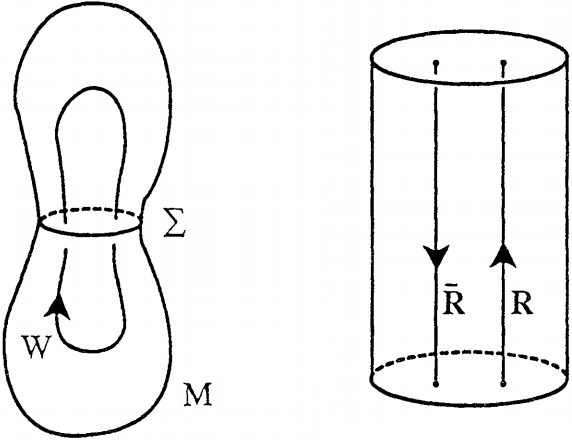
\includegraphics[width=0.5\textwidth]{figures/fig4_wilson_loop.png}
  \caption{左：一个含威尔逊圈 $W$ 的 3 维流形 $M$，沿黎曼面 $\Sigma$ 切开。右：切口处的领状邻域。曲面 $\Sigma$ 上有两个代表电荷的标记点，$W$ 的出射段与入射段在这两点插入表示 $R$ 与 $\bar R$ \cite{witten1989}。（原文 Figure 4，原文 p.24）}
  \label{fig:cut}
\end{figure}

\paragraph{提要}
% 原文标题：Synopsis.
每个可定向 3 维流形都可以沿一张 2 维曲面 $\Sigma$ 切成两块不相交的碎片。$\Sigma$ 作为可定向 2 维流形，可以赋予复结构，于是成为一张黎曼面。（$\Sigma$ 没有\textit{典范}复结构，这一点后面会变得重要。）切口附近，$M$ 的拓扑是 $\Sigma\times\R$；画面就像切一块瑞士奶酪。于是我们考虑这种拓扑的流形上的 CS 理论；把 $\R$ 当作时间方向，就得到与 $\Sigma$ 相配的希尔伯特空间 $\mathcal{H}_\Sigma$。一路上会遇到一个意外：高斯定律约束如今是非线性的。
% ==== 原文 p.25 ====
它使 $\mathcal{H}_\Sigma$ 成为有限维的。从精神上说，原因在于：$\mathcal{H}_\Sigma$ 来自理论的经典相空间，而这个相空间只由有限多个相位（phase）参数化，这些相位来自 $\Sigma$ 的拓扑所允许的非平凡威尔逊圈。我们也可以像以前一样，在 $M$ 里放纽结来加入源。其中有些纽结会穿过 $\Sigma$，于是出现图 \ref{fig:cut} 的画面。这时 $\Sigma$ 上带着若干“标记”点 $p_i$——纽结在此穿过——每个标记点附着相应威尔逊圈所给的表示 $R_i$。由这些数据构造 $\mathcal{H}_\Sigma$ 更为复杂，我们只勾勒做法。

% [Tutor Note: 物理图像] “有限多个相位”有来历：§2.3 的环面上相空间就是 $T^2$，两个威尔逊圈的和乐各是一个 $U(1)$ 纯相位；亏格 $g$ 时 $\pi_1(\Sigma)$ 有 $2g$ 个生成元，给出 $2g$ 个相位。
\begin{yizhu}[物理图像]
“由有限多个相位参数化”一句有来历。\S\ref{sec:2.3} 里环面上的经典相空间就是 $T^2$：$\pi_1(T^2)=\Z\oplus\Z$ 的两个生成元各给一个威尔逊圈，其和乐都是 $\mathrm{U}(1))$ 的纯相位，两个相位就是相空间的坐标。亏格 $g$ 的曲面同理给出 $2g$ 个相位。非阿贝尔情形还要加入色的数据，相空间随之升格为模空间。
\end{yizhu}

\subsection{全纯量子化}\label{sec:4.1}

\paragraph{正则形式}
% 原文标题：The canonical formalism.
我们从 $M=\Sigma\times\R$ 上的 CS 作用量 \eqref{eq:3.3} 出发。取规范 $A_0=0$，所得结果与 \S\ref{sec:2.3} 几乎一样，唯一区别是多了群论指标。作用量化为
\begin{equation}\tag{4.1}\label{eq:4.1}
  \SCS = \frac{k}{4\pi}\int_{\R}\dd t\int_{\Sigma}\dd^2 x\,\varepsilon^{ij}\Tr\bigl(A_i\dot A_j\bigr).
\end{equation}

% [Tutor Note: 易错点] (4.1) 与 (2.22) 逐字同形，只多一个 $\Tr$；系数 $k/4\pi$ 不含额外的 $1/2$。(2.20) 把同一作用量写成 $\frac{k}{2\pi}(\frac12\varepsilon^{ij}A_i\dot A_j+A_0B)$，那个 $1/2$ 已被 $k/2\pi$ 吸收。
\begin{yizhu}[易错点]
\eqref{eq:4.1} 是 \eqref{eq:2.22} 的非阿贝尔版：两式逐字同形，只多了一个 $\Tr$，系数就是 $k/4\pi$，\emph{不要}再补 $1/2$。核对看 \eqref{eq:2.20}：作者把同一作用量改写成 $\frac{k}{2\pi}\int(\frac12\varepsilon^{ij}A_i\dot A_j+A_0B)$，$1/2$ 是被 $k/4\pi\to k/2\pi$ 吸收掉的；在 \eqref{eq:4.1} 里再添 $1/2$，结果就差一倍。符号上取 $\varepsilon^{12}=+1$，则 $\varepsilon^{ij}A_i\dot A_j=A_1\dot A_2-A_2\dot A_1$，与 \eqref{eq:2.5} 的 $B=\varepsilon^{ij}\partial_iA_j$ 用同一约定。非阿贝尔情形下 $\Tr(A_i\dot A_j)$ 的两个因子不能交换，$\dot A_j$ 指 $\partial_tA_j$。
\end{yizhu}

和以前一样，哈密顿量为零，“坐标”是 $A_i$，“动量”是 $\varepsilon^{ij}A_j$。可见和以前一样，规范场与自己正则共轭。$A_\mu=(0,A_i^aT^a)$ 的空间分量满足正则泊松括号
\begin{equation}\tag{4.2}\label{eq:4.2}
  \bigl\{A_i^a(\mathbf{x}), A_j^b(\mathbf{y})\bigr\}
  = \frac{2\pi}{k}\,\varepsilon_{ij}\delta^{ab}\delta^{(2)}(\mathbf{x}-\mathbf{y}).
\end{equation}

% [Tutor Note: 易错点] (4.2) 与 (2.23) 有三处差别：多色指标 $a,b$ 与 $\delta^{ab}$（隐含正交基）；只给泊松括号，量子化后要补 $i$；$\varepsilon_{ij}$ 是下标，而 (4.1)(4.3) 用上标 $\varepsilon^{ij}$。
\begin{yizhu}[易错点]
\eqref{eq:4.2} 与 \eqref{eq:2.23} 的泊松括号相比有三处要看住。其一，右侧多了色结构 $\delta^{ab}$：这只在 $\Tr(T^aT^b)\propto\delta^{ab}$ 的正交基下成立，一般基底下应换成基灵型的逆 $K^{ab}$。其二，\eqref{eq:2.23} 把泊松括号与对易子并列，后者带 $i$；\eqref{eq:4.2} 只给经典括号，正则量子化后还得自己补 $i$。其三，这里的 $\varepsilon_{ij}$ 是下标，而 \eqref{eq:4.1}、\eqref{eq:4.3} 写的是上标 $\varepsilon^{ij}$；欧氏二维度规升降号不改分量，但抄录时不可随手改。
\end{yizhu}

这个关系定义了一个经典相空间，但它太大了：经典 CS 理论还受非阿贝尔高斯定律约束，此约束把我们限制在平坦联络上：
\begin{equation}\tag{4.3}\label{eq:4.3}
  \varepsilon^{ij}F_{ij}^a = 0 \quad\Longleftrightarrow\quad F = 0.
\end{equation}

% [Tutor Note: 易错点] $\varepsilon^{ij}F^a_{ij}=2F^a_{12}$：约束本身仍等价于 $F=0$，但因子 2 必须与 (2.21) 的 $B=F_{12}$ 及 (4.5) 的源项 $\frac{k}{4\pi}\varepsilon^{ij}F^a_{ij}$ 配套，丢了它就差一倍。
\begin{yizhu}[易错点]
$\varepsilon^{ij}F^a_{ij}=\varepsilon^{12}F^a_{12}+\varepsilon^{21}F^a_{21}=2F^a_{12}$，所以 \eqref{eq:4.3} 的左边是 $F^a_{12}$ 的两倍。因子 2 不改变“$=0$”这个结论（$F_{ij}$ 反对称，二维只有一个独立分量），但它必须与另外两式配套：\eqref{eq:2.21} 写的是 $\frac{k}{2\pi}B=\frac{k}{2\pi}F_{12}=0$；\eqref{eq:4.5} 写的是 $\frac{k}{4\pi}\varepsilon^{ij}F^a_{ij}=\sum_s\delta^{(2)}(x-x_s)T^a_s$。若把 \eqref{eq:4.3} 左边读成 $F^a_{12}$，\eqref{eq:4.5} 的源项就会差一倍。
\end{yizhu}

\paragraph{作战方案}
% 原文标题：Plan of attack.
由于 $F=\dd A+A\wedge A$ 对规范场是二次的，约束 \eqref{eq:4.3} 把非线性重新塞回 \eqref{eq:4.1}--\eqref{eq:4.2} 所定义的、本来极其自由的理论。要照 \S\ref{sec:2.3} 铺开的“先量子化、再约束”流程走，几乎不可能：在波泛函层面实施 \eqref{eq:4.3}（如 \eqref{eq:2.26} 那样），会得到一个严重非线性的偏微分方程，从而限死物理上允许的态。我们反过来做：“先约束、再量子化”，在经典层面就实施 \eqref{eq:4.3}。所得的相空间 $\mathcal{M}$ 称为平坦联络的\textit{模空间}；其元素是规范丛 $E\to\Sigma$ 上平坦主 $G$-联络 $A$ 的规范等价类。Atiyah 与 Bott \cite{atiyahbott1982} 研究过它，并证明：$\mathcal{M}$ 是紧致的、流形般的对象，只有温和奇点；它从 \eqref{eq:4.2} 的无约束相空间继承辛结构；实维数为 $d(2g-2)$，其中 $d=\dim G$，$g$ 是 $\Sigma$ 的亏格。又因 $\mathcal{M}$ 紧致，它的（辛）体积有限。依照海森堡不确定性原理，量子化通常在相空间的每单位体积产生一个量子自由度。于是我们看到，$\mathcal{M}$ 的量子化应当给出有限维的希尔伯特空间。

% [Tutor Note: 原文疑误] 原文 p.25 “It would be virtually impossible to follow the the “quantize, then constrain” procedure” 连写两个 the，属排印重复；译文按单次处理。
\begin{yizhu}[原文疑误]
原文此句作 “It would be virtually impossible to follow the the ‘quantize, then constrain’ procedure laid out in §2.3”，连写两个 the，属排印重复（原文 p.25）。译文按单次处理；若对照英文阅读，此处不必再找第二个定冠词。
\end{yizhu}

% [Tutor Note: 含糊点] $d(2g-2)$ 的来源是形变复形的上同调维数：不可约时 $H^0=0$，$\dim H^1=d(g-1)$，实维数加倍。Atiyah–Bott [21] 用指标定理算出；仅适用于 $g\ge2$ 的不可约部分。
\begin{yizhu}[含糊点]
维数 $d(2g-2)=2d(g-1)$ 是实维数，作者没有推导。它来自平坦联络形变复形的上同调：不可约联络满足 $H^0=0$，欧拉示性数 $d(1-g)$ 给出 $\dim H^1=d(g-1)$，实维数加倍即得。Atiyah--Bott \cite{atiyahbott1982} 用杨--米尔斯方程解空间的指标定理算出它，并说明奇点来自可约联络。该式只对 $g\ge2$ 的不可约部分成立：$g=0$ 时模空间退化为单点，$g=1$ 时维数为 $2\operatorname{rank}G$（$G=\mathrm{U}(1))$ 时就是 $T^2$），公式分别给出负值与零。
\end{yizhu}

% ==== 原文 p.26 ====
\paragraph{几何量子化}
% 原文标题：Geometric quantization.
在量子力学中 \cite{woodhouse}，我们通常从相空间 $\mathcal{P}$ 出发，它由坐标 $q^i$ 与动量 $p^i$ 参数化；然后把希尔伯特空间 $\mathcal{H}$ 定义为 $q^i$ 的复值平方可积函数空间。这个构造有两个显著特征：它要求把相空间变量拆成坐标与动量；并且它“挑出”其中一半坐标。（这种选择称为\textit{极化}。）我们可以用几何语言重写这个构造：在 $\mathcal{P}$ 的每一点附上一个复平面的副本，再把波函数 $\psi$ 定义为所得 $\C$-丛的任一截面（这个丛还没指定，马上会说），且满足两个条件。第一，$\psi$ 平方可积；第二，它只依赖 $q^i$、不依赖 $p^i$，即 $\partial\psi/\partial p^i=0$。坦白说，这个观点有点别扭——但别扭是故意的，因为接下来我们会看到它变得何等有力。

\paragraph{凯勒量子化}
% 原文标题：Kähler quantization.
\textit{凯勒流形}同时是辛流形、复流形与黎曼流形，三种结构彼此相容。\footnote{在某种意义上，它是一个相空间（因为它是辛的），却像一个弯曲的希尔伯特空间（因为它是复的，且带有切空间内积）。说得更直白些：凯勒流形就是一个花哨的甜甜圈。}
若相空间 $\mathcal{P}$ 恰好是凯勒的，我们就可以用新变量 $z^i=q^i+ip^i$ 与 $\bar z^i=q^i-ip^i$ 来参数化它。上面的 $\C$-丛变成 $\mathcal{P}$ 上的复线丛 $L$；我们只接受那些依赖 $z^i$、不依赖 $\bar z^i$ 的截面 $\psi\colon\mathcal{P}\to L$ 充当波函数。于是希尔伯特空间就定义为 $L$ 的\textit{全纯截面}空间。这类截面满足 $\partial\psi/\partial\bar z^i=0$，因此 $L$ 上的 $\bar\partial$ 算子湮灭它们。至于“平方可积性”，那需要一个内积。给 $L$ 配一个厄米度规就能算内积，例如 $\langle\psi|\psi\rangle$。厄米度规在 $L$ 上确定唯一的联络（其实就是列维--奇维塔联络！），称为\textit{陈联络} $\mathcal{A}$；它与 $\mathcal{P}$ 上的凯勒结构以两种方式相容。第一，由 $\mathcal{A}$ 构造的协变导数 $\mathcal{D}$ 与 $\bar\partial$ 算子相同，故物理波函数是协变常数的：$\mathcal{D}\psi=0$。第二，$\mathcal{A}$ 的曲率 $\Omega$ 满足 $\Omega=-i\omega$，其中 $\omega$ 就是（！）$\mathcal{P}$ 上的辛形式。接下来是一个奇迹：线丛的第一陈类 $c_1(L)=[\frac{i}{2\pi}\Omega]$ 是拓扑不变量，唯一地刻画 $L$。于是只要 $\mathcal{P}$ 的辛结构给定，所需的线丛就唯一确定了。

% [Tutor Note: 易错点] $\Omega=-i\omega$、$c_1(L)=[\frac{i}{2\pi}\Omega]$、$c_1(L)=[\frac{\omega}{2\pi}]$ 三式一致：$\frac{i}{2\pi}(-i\omega)=\frac{\omega}{2\pi}$。把 $-i$ 记成 $+i$ 会使 $c_1$ 变号、$\Omega$ 失去正定性。
\begin{yizhu}[易错点]
$\Omega=-i\omega$ 与两个陈类表达式是同一件事：代入即得 $\frac{i}{2\pi}\Omega=\frac{i}{2\pi}(-i\omega)=\frac{\omega}{2\pi}$。若把 $\Omega=-i\omega$ 的 $-i$ 记成 $+i$，$c_1(L)$ 整体变号，$\Omega$ 也不再正定。这里 $\omega$ 取实辛形式，$\Omega$ 是 $(1,1)$-形式；符号约定与陈类定义 $c_1=\frac{i}{2\pi}\Tr F$ 绑死。
\end{yizhu}

于是总结如下：设 $\mathcal{P}$ 是辛形式为 $\omega$ 的凯勒流形，取第一陈类为 $c_1(L)=[\frac{\omega}{2\pi}]$ 的线丛 $L$，今后称之为 $\mathcal{P}$ 的\textit{前量子线丛}。给 $L$ 配上陈联络；它确定 $L$ 上的厄米内积，曲率为 $\Omega=-i\omega$。那么与 $\mathcal{P}$ 相配的希尔伯特空间 $\mathcal{H}$ 就是 $L$ 的全纯截面空间；若 $\mathcal{P}$ 紧致，则 $\mathcal{H}$ 有限维。

\paragraph{希尔伯特空间}
% 原文标题：The Hilbert space.
回到本例：相空间 $\mathcal{P}=\mathcal{M}$ 并不带自然的复结构或凯勒结构。然而可以证明：一旦在曲面 $\Sigma$ 上选定复结构 $J$，模空间 $\mathcal{M}=\mathcal{M}_J$ 也就继承了复结构与凯勒结构。粗略地说，做法是先把规范群 $G$ 复化为 $G_\C$，然后（呼应上面的全纯量子化）在 $G_\C$ 中选一片“切片”，迫使复化规范丛上的联络全纯地变化。

% [Tutor Note: 含糊点] “it can be shown ... $\mathcal{M}_J$ inherits complex and Kähler structures” 省掉两步：复化 $G_\C$ 后平坦联络等价于全纯结构（Narasimhan–Seshadri / Kobayashi–Hitchin 对应）；切片把复化空间切回实子流形，Atiyah–Bott 的辛形式配上复结构给出凯勒结构。
\begin{yizhu}[含糊点]
此处 “it can be shown” 吞掉了两步论证。第一步，$G$ 复化为 $G_\C$ 后，“$G_\C$-联络的复规范等价类”与“$E$ 上的全纯结构 $\bar\partial_A$”是同一件事：次数为零的稳定全纯丛对应不可约平坦酉联络，即 Narasimhan--Seshadri 定理，其高秩推广为 Kobayashi--Hitchin 对应（$G=\mathrm{SU}(N)$ 时又称 Donaldson--Uhlenbeck--Yau 定理）。第二步，“取切片”把复化后的联络空间切回实子流形；$\mathcal{M}_J$ 的凯勒结构由 Atiyah--Bott \cite{atiyahbott1982} 的辛形式配上这个复结构给出。原文对这两步都未标文献。
\end{yizhu}

% ==== 原文 p.27 ====
一旦做出这个选择，$\mathcal{M}_J$ 从 \eqref{eq:4.2} 继承的辛形式 $\omega$ 就确定了第一陈类为 $c_1(L)=[\frac{\omega}{2\pi}]$ 的唯一线丛 $L$。接着用 $L$ 上的陈联络构造协变导数 $\mathcal{D}$，它与 $L$ 上的 $\bar\partial$ 算子一致；正是后者定义了全纯截面，而这些截面终于把希尔伯特空间 $\mathcal{H}_\Sigma^{(J)}$ 赋予 $\Sigma$。这番讨论坦白说相当抽象，但我们会在 \S\ref{sec:4.3} 看到一些例子。

当 $G=\mathrm{SU}(N)$、$k=1$ 时，$L$ 有一个稍具体的描述：基本想法是用 $\Sigma$ 上 $\bar\partial$ 算子产生的一族算子来构造 $L$。回忆取 $A_0=0$ 规范后，规范丛 $E\to M$ 可以看作 $\Sigma$ 上的丛。一旦固定 $\Sigma$ 上的复结构、把规范群复化为 $G_\C$、再选定 $G_\C$ 的一个表示（比如基础表示），$E$ 就获得 $\Sigma$ 上全纯向量丛的结构。$\mathcal{M}_J$ 的每一点是 $E$ 上的平坦联络；由该联络构造的协变导数保留了 $E$ 上复结构的部分信息。事实上，我们可以用它去“扭” $\Sigma$ 上本来就有的 $\bar\partial$ 算子——那是 $\Sigma$ 自身复结构给的。这样，$\mathcal{M}_J$ 就参数化 $E$ 上一族被扭的 $\bar\partial$ 算子。

\paragraph{行列式线丛}
% 原文标题：The determinant bundle.
现在有一种漂亮办法，给每个被扭的 $\bar\partial$ 算子（也就是 $\mathcal{M}_J$ 的每一点）配一条复线，从而得到前量子线丛。该构造由 Quillen \cite{quillen1986} 引入，做法基本上是“取 $\bar\partial$ 的行列式”。人们把行列式看作“取 $E$ 的最高外幂”这一操作的替身；最高外幂给出一个一维空间，当作一条线。更确切地说，给每个 $\bar\partial$ 算子配上一条线
\begin{equation}\tag{4.4}\label{eq:4.4}
  \mathcal{L}_{\bar\partial}
  = \bigwedge^{n}(\ker\bar\partial)^{*}\otimes\bigwedge^{n}(\operatorname{coker}\bar\partial).
\end{equation}
最后，把这些线粘起来，就定义了 $\mathcal{M}_J$ 上的\textit{行列式线丛} $L$。

% [Tutor Note: 易错点] (4.4) 的 $n$ 是 $\ker\bar\partial$ 的维数，不是 $E$ 的秩、也不是固定的外幂阶数；两侧同写一个 $n$ 隐含指标为零。取对偶的是 $\ker$ 一侧，换到 $\operatorname{coker}$ 一侧则 $c_1$ 变号。
\begin{yizhu}[易错点]
\eqref{eq:4.4} 的 $n$ 是 $\ker\bar\partial$ 的维数（两侧写同一个 $n$，隐含 $\dim\ker=\dim\operatorname{coker}$，即指标为零），不是 $E$ 的秩，也不是一个固定的外幂阶数。按黎曼--罗赫，$\operatorname{ind}\bar\partial_E=\deg E+\operatorname{rank}E\,(1-g)$；平坦联络给出 $\deg E=0$，但 $\operatorname{rank}E\,(1-g)$ 一般不为零，此时两侧维数并不相等，Quillen 的标准约定是取极大外幂。另外，取对偶的是 $\ker$ 这一侧：改到 $\operatorname{coker}$ 一侧，得到的就对偶线丛，$c_1$ 与曲率整体变号。
\end{yizhu}

% [Tutor Note: 含糊点] “狄拉克行列式给出厄米度规” 背后是 \$\\ 的模长按 $\exp(-\frac12\zeta'(0))$ 定义；Quillen [23] 把它与 $L^2$ 度规合成行列式线丛上的厄米度规，并证明曲率为 $-i\omega$。
\begin{yizhu}[含糊点]
“狄拉克行列式给出厄米度规”背后是 \$\\ 的行列式不是有限维行列式，其模长按 $\exp(-\frac12\zeta'(0))$ 定义，$\zeta$ 取自 $\bar\partial^*\bar\partial$ 的非零谱。Quillen \cite{quillen1986} 用它配上 $L^2$ 度规，在行列式线丛上定义厄米度规（今称 Quillen 度规），并证明该度规的曲率恰为 $-i\omega$、第一陈类为 $[\frac{\omega}{2\pi}]$。这正是“行列式线丛就是前量子线丛”的实质。
\end{yizhu}

可以验证：当 $k=1$ 时，这就是正确的线丛。狄拉克行列式在 $L$ 上给出厄米度规并确定陈联络，从而可以算出它的曲率与第一陈类。这件事由 Quillen 完成；他证明两者都符合 $c_1(L)=[\frac{\omega}{2\pi}]$ 与 $\Omega=-i\omega$，与辛形式 \eqref{eq:4.2} 一致。当 $k\neq1$ 时，行列式线丛 $L$ 把辛形式算错了一个因子 $k$；一般说来，能级 $k$ 上正确的线丛是 $L^{\otimes k}$。而当 $G\neq\mathrm{SU}(N)$ 时，出现的则是 $L^{\otimes k}$ 的某个（可能很大的）张量幂，这要归功于小平嵌入定理。

% [Tutor Note: 含糊点] 小平嵌入定理：紧复流形上正线丛（$c_1>0$ 的 ample 丛）的足够高张量幂给出到射影空间的嵌入。作者只说“某个（可能很大的）张量幂”，既不给幂次也不给构造，原文亦未标文献编号。
\begin{yizhu}[含糊点]
小平嵌入定理（Kodaira）说：紧复流形上若存在正线丛（$c_1>0$ 的 ample 线丛），则它的足够高张量幂给出到射影空间的嵌入。作者借它论证：$G\neq\mathrm{SU}(N)$ 时，前量子线丛未必是行列式线丛本身，而是其某个高次张量幂。这一步只保证存在性，幂次多大、线丛具体如何构造，原文都未说明，也未标出该定理的文献编号（标准出处为小平 1954）。
\end{yizhu}

\paragraph{模函子}
% 原文标题：The modular functor.
现在回到一个已反复出现的主题：$\Sigma$ 上没有典范的复结构。事实上，这类复结构 $J$ 在它们自己的黎曼面模空间里变动，我们记作 $\mathcal{M}_\Sigma$。从物理上讲，上面构造的希尔伯特空间 $\mathcal{H}_\Sigma^{(J)}$ 不能依赖复结构 $J$。理由在于：$\mathcal{H}_\Sigma^{(J)}$ 是一个问题的解，而该问题的提法只依赖可定向曲面 $\Sigma$，不依赖它的复结构。一个理论没有资格“知道” $J$，改变 $J$ 就不该影响它的希尔伯特空间。

% ==== 原文 p.28 ====
于是我们可以把各个 $\mathcal{H}_\Sigma^{(J)}$ 看作某个向量丛在模空间 $\mathcal{M}_\Sigma$ 上的纤维；这个丛的底点就是 $\Sigma$ 上的复结构 $J$。各纤维既然全同，丛就应当容许一个平坦联络，把纤维典范地等同起来。于是可以用 $\mathcal{H}_\Sigma$ 代替 $\mathcal{H}_\Sigma^{(J)}$，并得到一个映射：把曲面 $\Sigma$ 送到它的 CS 希尔伯特空间 $\mathcal{H}_\Sigma$。模空间上的这类平坦丛由 Segal \cite{segal} 研究过；他把映射 $\Sigma\mapsto\mathcal{H}_\Sigma$ 称为\textit{模函子}。

% ==== 片段汇报（s04a-hilbert） ====
% 覆盖：原文 p.24（§4 标题、Into the fray、图 4、Synopsis）—p.28（模函子段末，4.2 之前）。
% 编号公式：4 个，(4.1)--(4.4)，\tag 锁定。
% 图：图 4（figures/fig4_wilson_loop.png，width=0.5\textwidth，label=fig:cut），图注全译。
% 脚注：第 8 条（p.26）全译，位于“三种结构彼此相容”之后。
% 译注：12 条（易错点 6、含糊点 4、原文疑误 1、物理图像 1）。
% 记号裁定：图注 “R and R̄” 为 $\bar R$（PDF 中 R 上横线，非 $R^*$）。
% 维数裁定：$d(2g-2)$ 只适用于 $g\ge2$ 不可约情形；$g=0$ 单点、$g=1$ 为 $2\operatorname{rank}G$。
% 疑误：(a) p.25 “the the” 排印重复，照译并批注；(b) (4.2) 的 $\varepsilon_{ij}$ 与 (4.1)(4.3) 的 $\varepsilon^{ij}$ 上下标不一致，照录并批注。
% 待确认：无。
